\section{Design}
\subsection{TCP/IP}
%1 pourquoi utiliser xml, tcp, ip ... consomme de la batterie + UDP pas fiable ?
\begin{frame}
 \frametitle{Design et implications}
 Au lieu d'utiliser des données brutes, utiliser TCP/IP.\\
 \vspace{5mm}
 \textbf{$\rightarrow$} Accès à de nombreux outils disponibles \\
 \textbf{$\rightarrow$} Plus de chances d'être accepté par la communauté.\\
 \vspace{5mm}
 Mais tout cela crée de l'overhead, ce qui semble inapproprié pour un capteur aux ressources limitées. On verra des astuces qui permettront de réduire considérablement la taille des paquets envoyés.
\end{frame}
%utiliser une encapsulation tcp/ip augmente fortement la taille du message (40 octets) + inserer tableau
\begin{frame}
\frametitle{TCP/IP overhead}
L'encapsulation TCP/IP augmente la taille des paquets (le header fait 40 octets).\\
\vspace{5mm}
\begin{center}
\begin{tabular}{|c|c|c|c|}
\hline
~ & Minimum & Avec TCP/IP & TCP/IP\\
~ & requit & ~ & overhead\\
\hline
Paquets & 2 & 8 & 300\% \\
Octets & 11 & 338 & 2793\% \\
Délai (ms) & 6 & 375 & 6150\% \\
\hline
\end{tabular}
\end{center}
\end{frame}
%inserer figure 3
\begin{frame}
 \frametitle{Latences TCP/IP}
 \begin{figure}
  \centering
  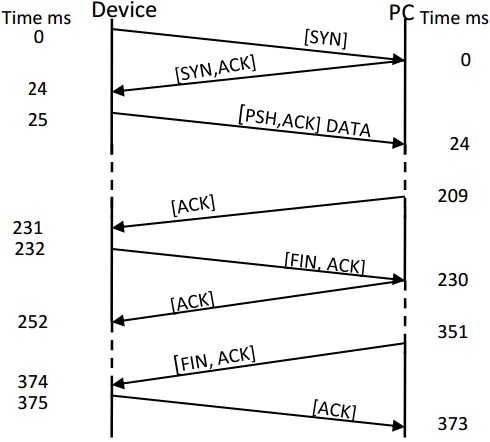
\includegraphics[scale=0.5]{figures/TCPlatences.jpg}
  \caption{Latences TCP}
  \label{tcplatences}
 \end{figure}
\end{frame}
%TCP persistante
\begin{frame}
 \frametitle{connexion TCP persistante}
 Sur la figure \ref{tcplatences} on observe qu'à chaque transmission, deux handshakes (début et fin) sont transmis. Or les capteurs communiqueront toujours qu'avec un seul autre appareil.
 %Dans l'application qu'ils utilisent, les capteurs communiquent seulement avec le controleur.
 On peut donc garder une connexion TCP persistante.\\
 \vspace{5mm}
 Ainsi, seul deux transmissions auront lieu lors du transfert d'un message: \texttt{[PSH,ACK]DATA} et \texttt{ACK}.
\end{frame}
%delayed ACK désactivé + figure
\begin{frame}
 \frametitle{1 ACK par message}
 \begin{figure}
  \begin{minipage}[c]{.46\linewidth}
 Habituellement, lors du transfert de données par TCP, le receveur envoie un ACK en communiquant le nombre d'octets reçus lorsqu'un timeout est écoulé. Et remet le timeout si tous les messages n'ont pas été transmis. Mais ici, puisqu'on transfert pratiquement toujours qu'un message, il est inutile d'attendre la fin du timeout pour l'envoi de l'ACK. Donc envoyons un ACK dès réception d'un paquet.
 \end{minipage}
 \begin{minipage}[c]{.46\linewidth}
  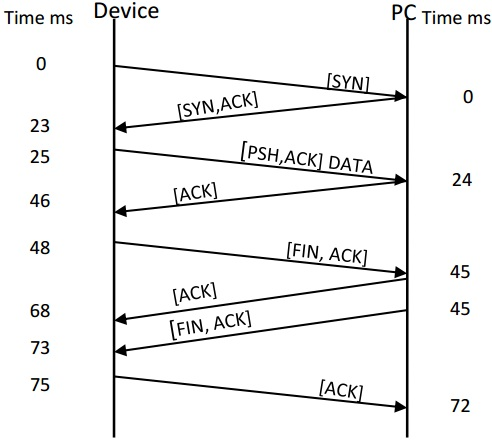
\includegraphics[scale=0.45]{figures/delayedACK.jpg}
  \caption{Délai ACK désactivé}
  \end{minipage}
 \end{figure}
\end{frame}
%retransmission pas bien + figure + on diminue fortement le timeout pour éteindre la radio le plus vite possible
\begin{frame}
 \frametitle{Retransmission}
 \begin{figure}
  \begin{minipage}[c]{.46\linewidth}
 Après écoulement d'un timeout, si le transmetteur ne reçoit pas d'ACK en retour du paquet qu'il a envoyé, il le retransmet. Et la probabilité de perte de paquet est d'autant plus grande pour une transmission sans fil.
 Le timeout généralement utilisé est beaucoup trop long pour un capteur. Pendant ce temps, la radio consomme de l'énergie.
 \vspace{3mm}\\
 Pour pallier à ce problème, il faut diminuer la valeur du timeout.
 \end{minipage}
 \begin{minipage}[c]{.46\linewidth}
  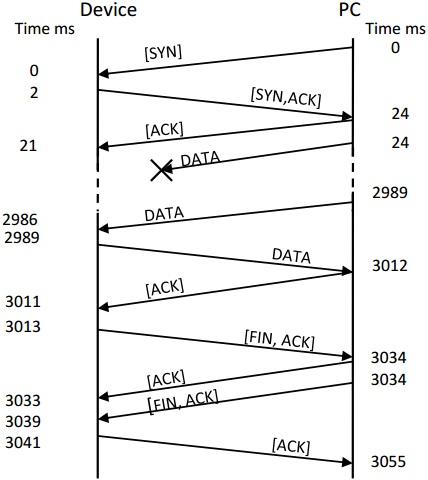
\includegraphics[scale=0.5]{figures/TCPretransmission.jpg}
  \caption{Retransmission}
  \label{retransmission}
  \end{minipage}
 \end{figure}
\end{frame}
%radio off entre les messages + valeur du temps minimum de dodo
\begin{frame}
 \frametitle{Sleep mode entre messages TCP}
 Si on observe la figure \ref{retransmission}, on s'aperçoit que pendant tout le transfert TCP, il y a encore une très grande partie du temps où la radio n'est pas utilisée.
 On pourrait éteindre la radio entre chaque transfert.
 Mais il faut pouvoir déterminer le temps minimum qu'il peut y avoir entre deux transferts.
 %Si la radio est éteinte plus longtemps que ce minimum, alors il loupe le paquet. Ce minimum dépend de la capacité du lien, nombre de noeuds à parcourir et taille du paquet.
\end{frame}

\begin{frame}
 \frametitle{6lowpan}
 Un datagramme IPv6 est trop volumineux pour un capteur sans fil.
 En effet, un paquet 802.15.4 ne supporte que 127 octets maximum.
 Mais il existe un autre protocole, le 6lowpan, qui permet de transférer un paquet IPv6 à travers plusieurs noeuds (mesh routing) avec des adresses plus courtes.\\
 \vspace{5mm}
 Le header du 6lowpan ne fait que 8 octets. (Celui de l'IPv4 en fait 20).
 Le controleur aura la charge de convertir les paquets 6lowpan en IPv6.
\end{frame}
\subsection{service web}
% duty cycle, il ne doit avoir transmission de message que lors de l'évenement.
\begin{frame}
 \frametitle{WS-eventing}
 Une large classe de capteur n'a besoin de transférer des messages que lors d'un événement (capteur de mouvement). Grâce au WS-eventing, le capteur peut entrer en sleep mode entre les événements.\\
 Le WS-eventing est composé de 5 entités fonctionnelles.
 \begin{enumerate}
  \item \textit{Event source} génère une interruption (détecteur de fumée)
  \item \textit{Event subscribers} sont Veulent être informé de l'événement.
  \item \textit{Subscription manager} accepte et gère les demandes d'inscriptions.
  \item \textit{Event subscription database} stocke les inscriptions actives.
  \item \textit{Notification manager} retransmet l'interruption à tous les intéressés enregistrés dans la base de donnée.
 \end{enumerate}
 %c'est comme le design patern observer
\end{frame}

\begin{frame}
 \frametitle{WS-eventing}
 \framesubtitle{Architecture}
 \begin{figure}
  \centering
  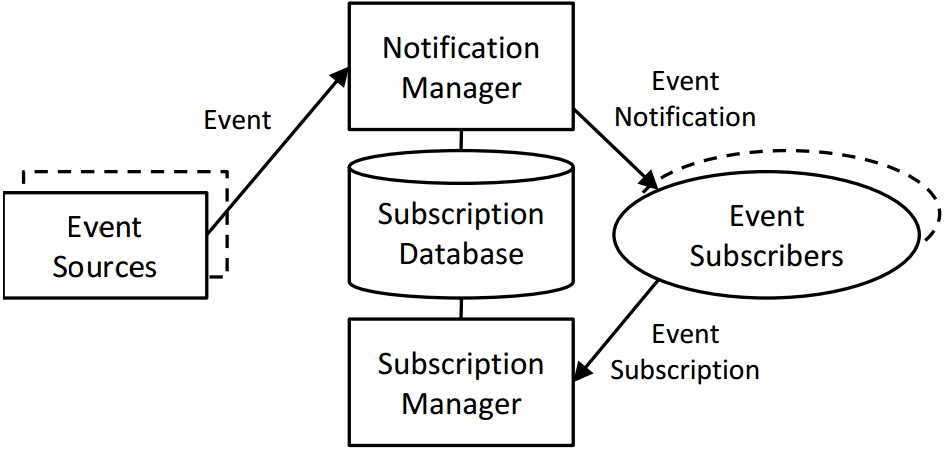
\includegraphics[scale=0.43]{figures/eventing.jpg}
  \caption{Architecture Web services eventing}
 \end{figure}
 Implémenté dans le contrôleur.
\end{frame}
%utilisation de fichier wsdl + expliquer ce que c'est + les protocoles disponible, on chois http
\begin{frame}
 \frametitle{WSDL}
 Un fichier WSDL décrit les méthodes disponibles sur le capteur. Nous développerons leur utilisation dans la section Prototypage.
 WSDL supporte trois protocoles pour les requêtes: SOAP, HTTP et MIME.\\
 \vspace{5mm}
 \begin{center}
 \begin{tabular}{|c|c|c|c|}
 \hline
 Nom de la méthode & SOAP 1.1 & SOAP 1.2 & HTTP\\
 \hline
 GetTemperature & 491 & 442 & 162\\
 GetTemperatureResponse & 479 & 499 & 258\\
 SetTemperature(70) & 528 & 482 & 202\\
 SetTemperatureResponse & 455 & 475 & 230\\
 \hline
 \end{tabular}
 \end{center}
 \vspace{5mm}
 On utilisera donc le protocole HTTP pour les requêtes.
\end{frame}
\subsection{XML}
%utilisation de xml. + tableau + expliquer chaque ligne du tableau.